\section{A first image}\label{sec:first-image}

Because nothing absorbs or scatters, a thermal gravitational image is a line
integral. Integrating Eq.~\eqref{eq:kirchhoff} over frequency for constant
$\eta$ gives the energy emitted per unit volume and solid angle,
$j_E = \alpha\sigma T^4/\pi$, where $\sigma$ is the Stefan--Boltzmann constant.
Dividing by the mean energy of a thermal quantum, $2.70\,\kB T$, gives a
number emissivity $j_N$, and the brightness of the pixel that looks along the
unit vector $\hat n$ is
\begin{equation}\label{eq:column}
N(\hat n) = \int_0^\infty j_N\bigl(s\,\hat n\bigr)\,\dd s ,
\end{equation}
in gravitons per second, per square metre of aperture, per steradian.

Figure~\ref{fig:sun-at-midnight} evaluates Eq.~\eqref{eq:column} for an
observer on the night side of the Earth, at latitude $40^\circ$ at local
midnight. The Earth is modelled as five uniform shells with rounded textbook
radii and temperatures, from a crust at $700\,\mathrm{K}$ to an inner core at
$5500\,\mathrm{K}$. Looking straight down, the line of sight runs through
$12{,}700\,\mathrm{km}$ of rock and iron, and the expected brightness is
$6\times10^{-5}$ gravitons per second per square metre per steradian. The
Sun radiates of order $10^{8}\,\mathrm{W}$ in gravitational waves
\cite{GarciaCelyRingwald2025,Steane2024}, about
$4\times10^{-16}\,\mathrm{W\,m^{-2}}$ at the Earth: roughly one graviton per
square metre per second, arriving from a patch of sky a tenth of a degree
across. Its surface brightness is some $10^{10}$ times that of the Earth's
interior in this model, so the Sun dominates the thermal gravitational sky by
day and by night.

Two assumptions carry most of the uncertainty. The Earth's internal friction
at thermal frequencies is not known to us, and is set to
$\eta = 10^{-3}\,\mathrm{Pa\,s}$ throughout as a placeholder. The Sun's
emission is spread uniformly over the inner fifth of its radius, where the
true profile is peaked toward the centre.

\paragraph{How faint.} The image is an expectation value. Figure~\ref{fig:budget}
sets the numbers of gravitons side by side. Only the Sun delivers enough for a
picture to assemble itself, graviton by graviton, within a human lifetime.

\begin{figure}
\centering
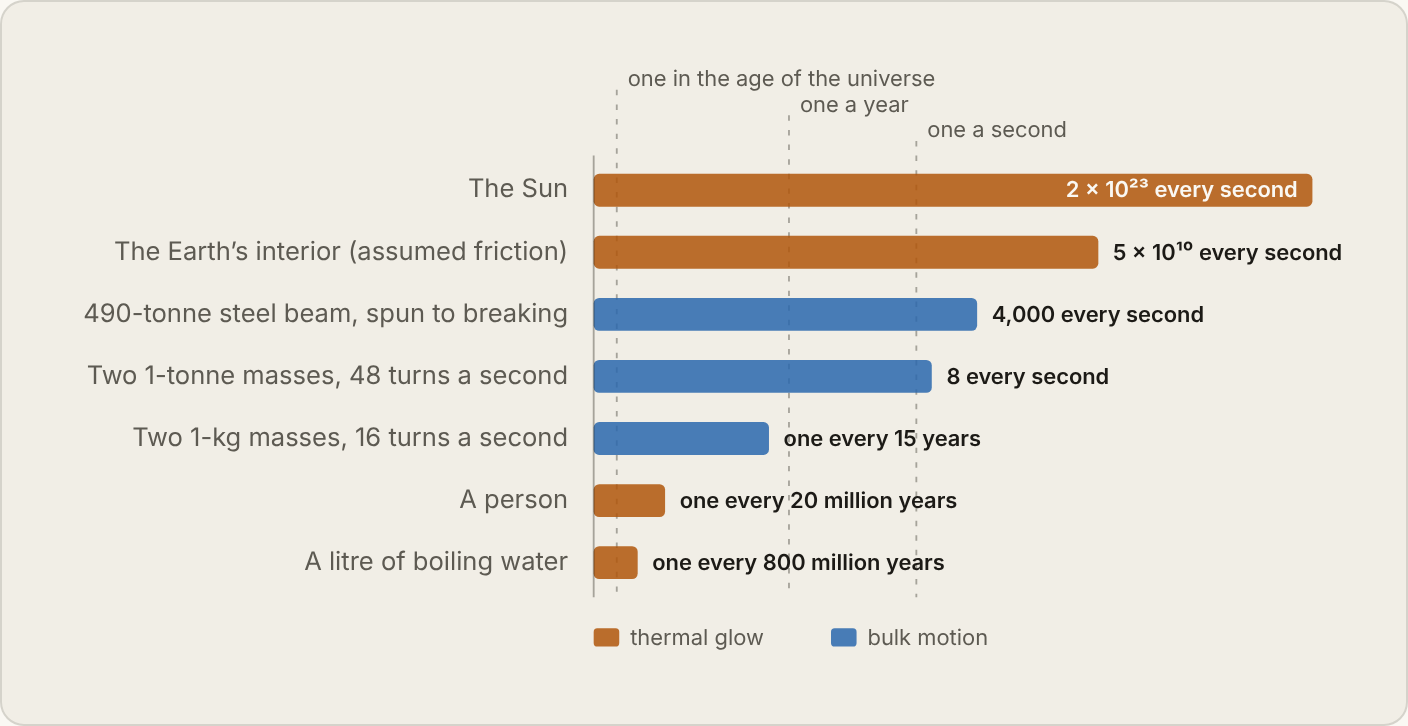
\includegraphics[width=\linewidth]{figures/budget.png}
\caption{Gravitons emitted per second by whole objects, on a logarithmic
scale spanning forty powers of ten. The spinning masses radiate by bulk
motion, Eq.~\eqref{eq:dumbbell}; the others thermally,
Eq.~\eqref{eq:kirchhoff}, with a constant friction that makes the thermal
values upper estimates. The Earth's value depends on its assumed
friction.}\label{fig:budget}
\end{figure}

All images shown with this paper are computed twice: by the engine that draws
them, and by an independent reference implementation that integrates
Eq.~\eqref{eq:column} by a different method. The two agree to a few parts in a
million along ordinary lines of sight.
